\documentclass[UTF8]{ctexart}

\title{面向对象技术与编程课程设计期末考试 \\ [2ex] \begin{large} 题目 10 宾馆房间管理系统 \end{large} }

\author{陈伯硕}
\date{\today}
\bibliographystyle{plain} % 声明参考文献格式

% 插图功能的相关宏包
\usepackage{graphicx}

% % 修改字体
% \usepackage{type1cm}  %(其中的 cm 为 Computer Modern 的缩写)
% \CJKfamily{song}  % 宋体

% 增加目录中的项目用tocbibind
\usepackage[nottoc]{tocbibind}
% 宏会默认增加目录本身,参考文献,索引等项目.noctoc取消了目录中显示目录
\begin{document}

\maketitle
\tableofcontents

\section{问题描述}
设计一个程序实现对宾馆房间的基本管理,可以实现:
客房信息的录入功能;客人入住
登记、客人退房结算;客房信息浏览功能,浏览全部客户的信息,客房信息和客户信息分别
保存于不同文件;客房信息查询,查询空房间情况,实现按房间号查询等。

\section{基本要求}
(1)至少包含四个类:Date 类(日期),客房 Room 类,主要包含客房信息(房号,类
型,是否有客人等)及相关操作;客人 Guest 类,主要完成客户信息(身份证,入住时间,
姓名,性别等)的相关操作;Manage 类实现对客房的管理。

(2)用文本编辑器编写一个 room.txt 的文件,文件中应包含 20 条以上记录(房间
的初始状态),再编辑一个 guest.txt 的文本文件,包含 10 条以上客人记录。在运行程序时自动载入。

在(2)中为了数据处理方便, 替换成了csv文件
\section{需求分析}
设计程序模拟旅馆管理系统, 记录房间的使用情况和客人的住宿情况
% 以无歧义的陈述说明程序设计的任务,强调的是程序要做什么?
% 并明确规定:
% 输入的形式和输入值的范围;
% 输出的形式;
% 程序所能达到的功能;测试数据:
% 包括正确的输入及其输出结果和含有错误的输入及其输出结果。
\section{概要设计}
说明本程序中主程序的流程以及各程序模块之间的层次(调用) 关系。
\section{详细设计}
% 实现概要设计中定义的所有数据类型,给出关键部分源程序的清单,要求程序有充分的注释语句,至少要注释每个函数参数的含义和函数返回值的含义。

\subsection{date 类}

类似于课本\cite{textbook}的date类的实现如图\ref{fig:date}

  % figure 环境,就是插图使用的浮动体环境,相当于普通段落,没有缩进
  \begin{figure}% 可选参数ht表示可以出现在文字所在处(here)或顶部
    \centering% 后面内容居中
    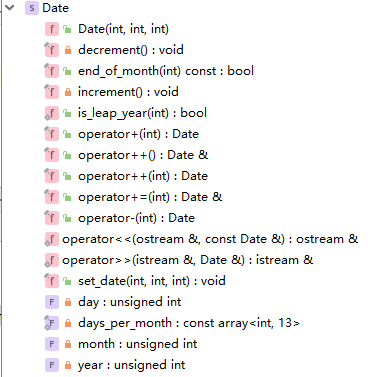
\includegraphics[scale = 1]{structure_date.png}
    % \includegraphics有两个参数,方括号中的可选参数设定了宽度
    % 可选参数有[scale=放缩因子][height=高度][width=宽度]
    % 第二个参数是文件名,放在源文件目录
    \caption{date 结构图}% 给插图加上编号和标题
    \label{fig:date}
  \end{figure}
\subsection{Room 类}

简单的room实现如图\ref{fig:room}

% figure 环境,就是插图使用的浮动体环境,相当于普通段落,没有缩进
  \begin{figure}% 可选参数ht表示可以出现在文字所在处(here)或顶部
    \centering% 后面内容居中
    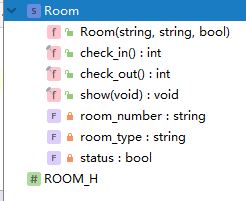
\includegraphics[scale = 1]{structure_room.png}
    % \includegraphics有两个参数,方括号中的可选参数设定了宽度
    % 可选参数有[scale=放缩因子][height=高度][width=宽度]
    % 第二个参数是文件名,放在源文件目录
    \caption{room 结构图}% 给插图加上编号和标题
    \label{fig:room}
  \end{figure}

\section{调试分析}
内容包括: 调试过程中遇到的问题是如何解决的以及对设计与实现的回顾
讨论和分析;
\section{用户使用说明}
说明如何使用你编写的程序,详细列出每一步的操作步骤。
\section{测试结果}
设计测试数据,或具体给出测试数据。要求测试数据完整和严格,能全面地
测试所设
计程序的功能。
\section{程序设计总结}

\nocite{Lippman:2012:CP:2423877}% 只在参考文献中显示,不直接引用
\bibliography{reference} % 提示从reference数据库获取文献信息,来打印参考文献

\end{document}
